\section{The AMIDST requirements engineering process}
\label{sec:AmidstRequirementProcess}

This section contains a description of the AMIDST RE process.  We first give a brief overview of AMIDST and describe the 
main characteristics of the AMIDST project that has influenced and shaped the RE process. Based on these characteristics 
we present the AMIDST RE process, which is based on the RE processes described in Section~\ref{sec:use-case-driven}, 
but tailored to the specific characteristics of AMIDST. Since the focus of the present RE process is on the functionality and 
documentation of the software products being developed, we will, e.g., not cover process-related requirements or non-
functional requirements, c.f.\ Section~\ref{sec:use-case-driven}. Non-functional requirements are defined by the
aforementioned DoW. 

\subsection{The AMIDST project: a brief overview}

AMIDST is a project funded by the European Union's Seventh Framework Programme for research technological development
and demonstration. The objective of AMIDST is to develop a scalable toolbox capable of providing a framework that
facilitates efficient prediction and data analysis in streaming data. The toolbox will be instantiated to target three
distinct industries represented by the three industrial use case providers in the AMIDST consortium. The use case
provider in the energy domain is Verdande Technology, the use case provider in the financial domain is the Cajamar Cajas
Rurales Unidas, and the use case provider in the automobile domain is Daimler AG.  In addition to the use case
providers, there are also three academic partners and a fourth industrial partner in the software industry.  The fourth
industrial partner is Hugin Expert and the three academic partners are the Norwegian University of Science and Technologogy, Universidad de Almeria, and Aalborg University.

The development of the toolbox and its subsequent instantiation will be driven by functional requirements specified by the use case providers and elicited in accordance with the RE process described in the present document; the requirements supplement the non-functional requirements described in the DoW framework. If deemed effective, the instantiated toolboxes (referred to as AMIDST \emph{solutions}) will be adopted by the use case providers. 

The AMIDST project is structured around ten work packages. The first work package is concerned with requirements
engineering and evaluation. Work packages 2--4 focus on methodological developments to be applied on the massive data streams.  In particular, there is emphasis on probabilistic models as well as scalable inference and learning
algorithms tailored to these models. Work package 5 is concerned with extensions to the AMIDST solutions to the Hugin software toolbox, which is already commercially available.  In Work packages 6--8 the AMIDST solutions for the three industrial partners will be realised. Finally, Work packages 9 and 10 deal with dissemination and exploitation as well as management.     

\subsection{Characteristics of the AMIDST project}
\label{sec:characteristics}

In this section we identify and describe the key characteristics of the AMIDST project that directly influence the 
requirements
engineering process. 

\ \\
\noindent \emph{Characteristics one:  Pre-specified scope of the project}
\label{sec:characteristic1}

The AMIDST project is funded by the European Union's Seventh Framework Programme for research, technological
development, and demonstration. The overall scope and main developments in the project are therefore defined from the
beginning of the project period and documented in the Description of Work. This will henceforth be referred to
as the DoW framework. More detailed requirements pertaining
to the functionality and documentation of the developed software should thus fit within the DoW framework, and their
necessity in relation to AMIDST should be justified and demonstrated.   


 

\ \\
\noindent \emph{Characteristics two: Partners at different geographical locations}
\label{sec:characteristic2}

The AMIDST consortium consists of 7 partners/stakeholders, 4 industrial and 3 universities, which are situated in 4 different
countries. This diverse consortium composition has at least a two-fold impact on the RE process.

First of
all, although AMIDST targets the industrial stakeholders' common need for processing massive data streams, the more
intrinsic aspects of the three industrial domains differ significantly. This, in turn, means that the partners will have different
(possibly conflicting) requirements for the system being developed. To ensure that the requirements are comparable
across domains and abide to the DoW, a unified formal framework for eliciting system requirements is needed. Such a
framework may also provide transparency in the overall requirement engineering process and help prioritize requirements
across different domains and thereby help resolve potential conflicts.   

Secondly, with the project partners located in different countries, there is a need for a controlled and stringent requirements
process in order to limit travel expenditures. This approach is supported by a unified formal requirements
engineering framework. Consultancy and discussions in relation to the
requirements will primarily be achieved through telecommunication conferences and by physical meetings only secondarily. 
% 
%% The result is a project with many stakeholders, which have different backgrounds, priorities and influences on the 
%software. Moreover, the partners are located in different countries, which implies that the financial and time costs for 
%personal meetings are quite high.  This characteristic has an influence on the pursued RE process, because the process is 
%restricted to not rely heavily on meetings with many participants.

\ \\
\noindent \emph{Characteristics three: Transfer of domain knowledge between partners}
\label{sec:characteristic3}

The industrial partners of the AMIDST project come from very different domains: the automotive, energy, and finance
industry. To ensure the development, refinement, and completion of the unified formal requirements framework it is
necessary with regular and structured communications among the project partners during the RE
process. This not only relates to the specific requirements, but also to the software and user context in which the
AMIDST framework should be deployed. The latter part, in particular, is required for a proper evaluation and validation
of the elicited requirements.


% On one side, it was essential that the industrial partners gained enough insight of what can be done with
% probabilistic graphical models to identify proper use cases.  On the other side, it was essential that the academic
% partners gained enough knowledge about the industrial domains to understand the proposed use cases and 
%requirements. 
%This was considered in the way we divided our work among the academic partners. 

\ \\
\noindent \emph{Characteristics four:  One framework for three different domains}
\label{sec:characteristic4}

The AMIDST toolbox should define a general framework that can encompass the diverse domains of the three industrial
partners. Thus, the format of the unified requirements framework should be sufficiently general and flexible to
allow for all relevant requirements to be elicited for the three domains. At the same time the framework should be
appropriately structured and formalized enabling a controlled elicitation process (see also Characteristic two) with the
requirements specified in a consistent manner making them comparable across domains. In order to also provide a basis 
for a controlled and
balanced system development, the requirements should be linked to
relevant project phases, work packages, and tasks. This, in particular, will provide the work package leaders with
a clear overview of the requirements that are relevant for the activities in a specific work package.   
%
%%One single framework shall solve all posed problems.  It is therefore a challenge to find common requirements that are 
%addressing problems across all three domains.
%

\ \\
\noindent \emph{Characteristics five: Potential refinement of project focus}
\label{sec:characteristic5}

AMIDST is an RTD project, where both the industrial and academic partners' understanding of the domains develop as
the project unfolds. In order to support a potential refinement of the project's focus and goals, the requirements
engineering process should allow for an internal (re)prioritization of the requirements that is transparent across
application domains.    


% The posed problems are challenging and, as usual, some aspects of the problems are not fully understood at this stage 
%in the project. We realize that the priority of some of the requirements can change as the project continue. There is also an 
%uncertainty related to how satisfied the industrial partners will be when the proposed solutions are implemented.  

%Defining a requirement is linked with the perception of which design pattern to follow \cite{Ral13}.  A design pattern is 
%chosen by the software %developer and is basically the path to meet the requirement.  As explained in \cite{Ral13}, when 
%there is a high degree of unclarity of which  design %pattern to follow, this ambiguity is transferred to the definition of the 
%requirement as well.  The goal of the AMIDST software is to reach targets %that are highly innovational, meaning that it is 
%particularly difficult to define requirements that are clear and unambiguous.
%

\subsection{Project phases and AMIDST requirements identification }

%% We decompose the overall project period into phases to better -> support identification of requirements and work
%% package allocation.

The overall project duration will be decomposed into different phases, each having distinct requirements. According to
\cite{Eig09} a project's life cycle can be divided into three general phases: the design phase, operations phase, and
disposal phase. The disposal phase is outside the scope of AMIDST and, thus, will not be considered in the present
document. The design and operations phase, however, represent the
temporal development of the project, and are initiated by the start of the project and ends with the testing of the
deployed system, which will be adopted by the use case providers if deemed effective. Each
phase can furthermore be described as a collection of distinct stages in the project. The overall process is
illustrated in Figure~\ref{REprocess2}. 

%
%%%In order for a requirement to be useful for the software engineers, they are often associated with steps in a product life 
%cycle as for instance described in \cite{Eig09}.  In this reference the overall life cycle is divided into three phases; design 
%phase, operation phase and disposal phase.  In the AMIDST software, the disposal phase is not relevant for us.  

\begin{figure}[htbp]
\centering
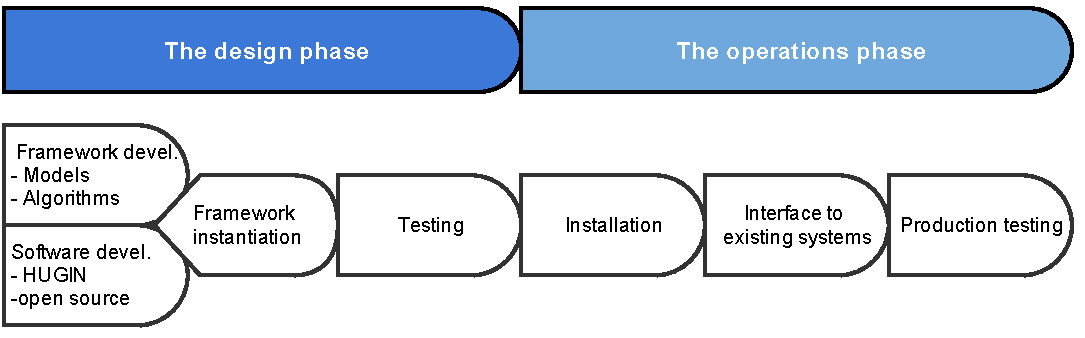
\includegraphics [keepaspectratio,width = 14cm] {amidst_phases}
\caption{The figure shows the key stages in the design and operations phases. For the requirement specification, each
  requirement should be defined relative to one of these stages.} 
\label{REprocess2}
\end{figure}


%\fixme{Describe the content of the two phases, design and operations}


In the design phase  general functionality requirements for the system are specified, i.e., what the system should do and 
support.
Figure \ref{REprocess2} details key stages inside this phase. The first stage consists of the design of the general
framework (models and algorithms) as well as the design and development of the software tools. These stages are 
primarily
related to Work packages 1--5. In the second stage, the general framework and software is instantiated for each specific
use case. Finally, initial tests of the use case instantiated frameworks are conducted.  During this phase of the project, 
possible design requirements could, e.g., address
\begin{itemize}[itemsep=2pt,parsep=2pt,topsep=4pt, partopsep=4pt]
 \item the scope of the model
 \item the interpretability of the learned models
 \item the extent and type of domain knowledge that can be integrated into the models
 \item prediction accuracy of the developed models
 \item documentation
\end{itemize}

The requirements for the operations phase concern the functionality of the deployed system. In Figure \ref{REprocess2}, 
we decompose this phase into three stages: installation, interface to existing systems, and production testing. The 
requirements for this phase could, e.g., address
\begin{itemize}[itemsep=2pt,parsep=2pt,topsep=4pt, partopsep=4pt]
 \item hardware constraints
 \item interfaces to existing software or data base systems
 \item inference functionality, i.e., what queries the system should be able to answer
 \item response time
\end{itemize}


\subsubsection{Use cases and user groups in the requirements engineering process}

As discussed in Section~\ref{sec:stateOfArt}, a use case driven approach to RE puts emphasis on
the functional requirements of the system, by focusing on the
interactions between actors (this being either persons or other hardware/software modules ) and the system. This focus
is consistent with the general objectives of the RE process in AMIDST, and the use case-based
approach to RE is therefore adopted in AMIDST. However, to obtain more well-defined
requirements and establish a closer connection
between the use cases and the project stages/work packages (c.f.\ Characteristics four), we further require that use
cases should be specified as indivisible scenarios. Specifically, when defining the use cases, 
the industrial partners were informed that:

\begin{quote}
\emph{  \ldots a use case should ideally be indivisible. If a use case can be decomposed into multiple
  sub-use cases, each with a well-defined sub-objective relevant for AMIDST, then these sub-use cases should be
  described separately.}
\end{quote}

The requirements derived from a use case are typically specified in relation to a particular user or type of user (possibly 
another
component of the system). In AMIDST the possible users have very diverse backgrounds, ranging from developers with an
intimate knowledge of the key technologies embedded in the AMIDST framework to programmers and users working in
marketing. In order to ensure that focus is on the future \emph{users} of the system, the AMIDST requirements
engineering process also adopts and identifies user groups (as described in Section~\ref{sec:stateOfArt}), which will be
explicitly linked to the relevant requirements.
%
%% A use case driven approach is chosen in the AMIDST RE process.  In a use case driven approach, there is a clear focus 
%on the functional requirements which are the most relevant to the user.  It is also important that requirement are listed with 
%respect to each use case, meaning that the users get a better overview than if requirements are listed component-wise. 
%The use case driven approach is designed to ease the communication between the user and the software developer.  It is 
%therefore a good choice to meet characteristic three.  
%
%%Moreover, since the functional requirements are generally more high-level, this approach comply with characteristic five.  
%This is because it is less likely to add a very specific requirement that becomes less relevant later.  
%
%%In order to meet characteristic one, the use case providers are asked to describe how every use case can be tested and 
%what is needed for them to deem the product a success.  These requirements are identified as performance requirements.

\subsection{The general AMIDST requirements engineering process}
\label{sec:reprocess}

To ensure a sufficient amount of knowledge transfer between the partners (c.f.\ Characteristics three, Page~
\pageref{sec:characteristic3}),
the overall  RE process will be carried out in an iterative fashion that is expected to involve a
high level of cooperation and interaction between the partners.  

In Figure \ref{REprocess1}, inspired by \cite{Ebe10}, an illustration of the RE process for AMIDST is given.  The process 
contains five phases, which are discussed below.

\emph{Preparation I:}  This phase starts at the same time as Work package 1 and ends when the initial template of the RE process is finished,
see Appendix A in \cite{Fer14}.  In this template, the RE process
is outlined, including definitions of use cases, user groups, and how to link requirements with the stages and WP/tasks
in the development process.  In order to meet characteristic three, four and five, the use case providers are asked to
provide a detailed description of the system context that the AMIDST solution is expected to operate in, identify user
groups, describe use cases and requirements.  In order to meet characteristic four, the requirements are linked to their
associated work packages and tasks. 

\emph{Elicitation:} The distribution of the above mentioned template marks the initialization of this phase.  Its aim is
to get an initial high-level description of the different use cases and their requirements. This information are
specified by the use case providers in collaboration with the academic partners, thus addressing characteristic one,
three and four.  Once the use case providers return the document with the requested information, feedback and
review sessions should be held to clarify and refine the information provided. These review sessions not only serve as a
quality check and to align the expectations of the developers/designers and use case providers, but they also provide the 
end-users with an
opportunity to give feedback to the developers.  At the end of the elicitation phase, the
aim is to have a first coherent description of the requirements for each use case provider. 

 \emph{Prioritization:} In this phase the use case providers complete and refine  the document template used in the
 previous phase. The provided template explicitly links each of the requirements to the relevant work packages and tasks in 
the
 AMIDST project, thus providing an initial consistency check with the DoW framework (see Characteristic one). Moreover, 
the template allows the use case providers to give
 a prioritization of the relevant requirements for the AMIDST framework.  Specifically, the use case
 providers are asked to rate each requirement in terms of whether it is a must, should, or could requirement:
\begin{description}
\item[Must (be)] These requirements are expected by the use case providers and include properties described in the 
AMIDST DoW framework.
\item[Should (performance)] These requirements are expected by the use case provider, but are not explicitly agreed upon.
\item[Could (delighters)] Optional requirements that will often be satisfying to have, but which have not been required
  by the use case provider in neither an explicit nor implicit manner.
\end{description}
 This high-level prioritization scheme is inspired by the Kano model
 correlating product development with customer satisfaction, see Figure~\ref{fig:kano}. Within each of these categories, the
 use case providers should also make a more fine-grained prioritization by numerically weighting the different
 requirements on a scale from 0 to 100. 

\begin{figure}[htbp]
  \centering
  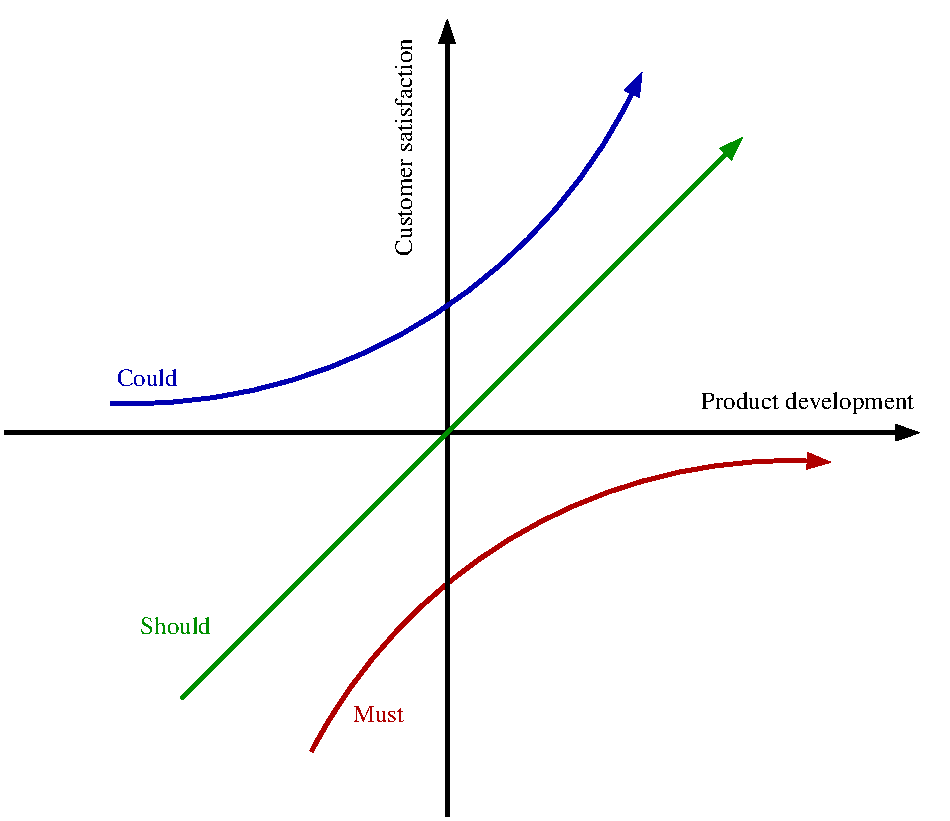
\includegraphics[width=0.65\linewidth]{kano}
  \caption{The Kano model.}
  \label{fig:kano}
\end{figure}


\emph{Validation:} In this phase, the requirements from all use case providers are collected to get the \emph{big
  picture}.  This includes a discussion among the members of the  project science review group as to the extend to which 
the
requirements can be accommodated and whether they collectively produce any potential conflicts, either internally or in
relation to the
DoW framework. Revisions and negotiations of the detailed requirements are therefore expected.  In this phase, it is 
important to ensure that Characteristic one is met.

 \emph{Evaluation and Testing:} In this phase, the focus is on the elicitation of the evaluation and testing procedures
 in the AMIDST project. This phase starts with the distribution of a new document template, where the aim is to obtain a
 high level description of the evaluation and testing methods that are necessary to measure the performance of the AMIDST
 framework. This phase is not strictly part of the RE process, but will supplement the process by providing
 detailed specifications of how to perform specific tests and evaluations. Documentation of this phase is out of the scope of 
the present document, but will
 be included in the initial version of the AMIDST handbook (Deliverable D1.3).    


\begin{figure}[htbp]
\centering
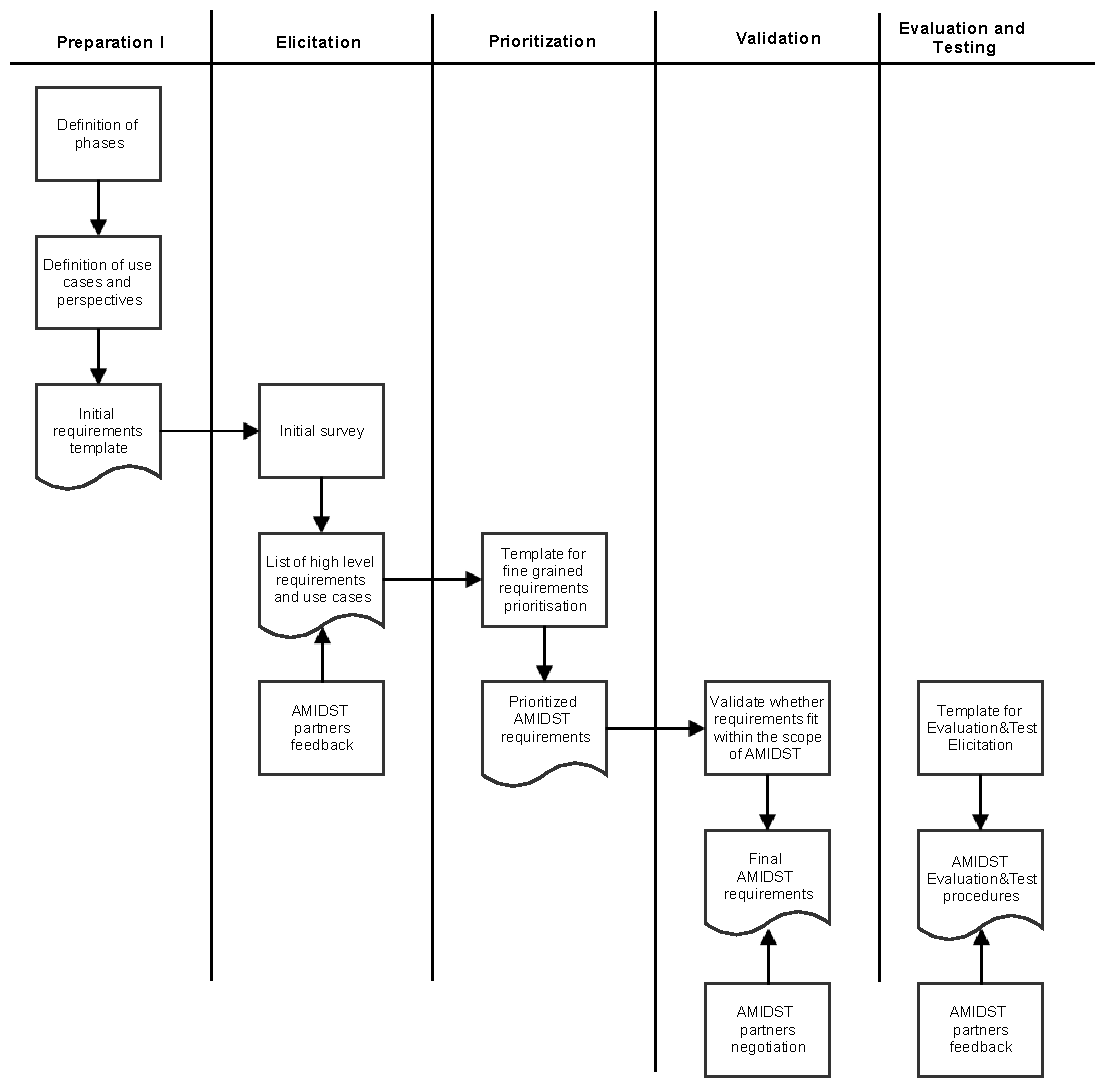
\includegraphics [keepaspectratio,width =\linewidth] {amidst_re}
\caption{Description of the five phases in the RE process in AMIDST.}
\label{REprocess1}
\end{figure}



% \subsection{Main aspects of the AMIDST's RE process}
% \label{sec:reprocess}
%
%% In this subsection, we detail the main elements that define the AMIDST RE process, which are strongly influenced by the 
%characteristics in the previous subsection.  This subsection contains a description of how the work is divided among the 
%partners and how the use case driven approach is adapted.  Moreover, a document template that is central in the AMIDST 
%RE process is described.  Requirement are discussed in terms of how they are linked with the product life cycle and 
%deliveries in the AMIDST project.  Prioritization of requirements are also briefly described, before the outline of the main 
%activities in the AMIDST RE process is given.
%


%%% Local Variables: 
%%% mode: latex
%%% TeX-master: "REproccess"
%%% End: 
